\section{Supplementary Methodology}
\label{app:method}

\subsection{Two Literatures Behind the Expectation}
\label{app:literatures}
Two established literatures make the expectation precise, and neither has been brought to bear on carrier-grid storage. The first is approximation-theoretic. The $L_2$ error of representing a continuous field by samples on a grid of step $T$ is governed, to leading order, by an error kernel whose decay is fixed by the representation's approximation order, so refining the step buys a predictable and bounded amount of accuracy rather than an arbitrary one~\cite{blu1999fourier,blu1999approximation}; the modern statement of sampling beyond the strictly band-limited case, which is the regime any real instrument occupies, is due to the same school~\cite{unser2000sampling}. On a field the instrument has already band-limited, refining the grid past the response width therefore adds samples whose values are very nearly determined by their neighbours.

The second literature says what a codec does with such samples. Wavelet coefficient magnitudes persist across scales, and it is that persistence which zerotree coders exploit implicitly~\cite{shapiro1993ezw,said1996spiht}; modelling it explicitly as a hidden Markov tree over the scale hierarchy~\cite{crouse1998hmt}, or coding each coefficient conditioned on its parent~\cite{buccigrossi1999joint}, turns the same structure into bits saved. An added octave carrying almost no variance is precisely the case those models handle best, which is why the oversampling penalty is expected to be much smaller than the factor of~\eqref{eq:alpha}, and why the question is quantitative rather than rhetorical. Section~\ref{sec:support_controls} bears on how little that octave carries, though it cannot settle it: a median of $0.21\%$ of each scene's variance lies above half the native Nyquist. That band, $0.025$--$\SI{0.05}{m^{-1}}$, is not the octave level~20 adds over level~19, which runs from $0.040$ to $\SI{0.080}{m^{-1}}$ and lies mostly \emph{above} the native product's own Nyquist. What the native raster can be asked is whether its own top half is nearly empty, and it is; whether the band beyond it is empty cannot be read off a product that does not represent it. It can be read off the carrier, and Section~\ref{sec:level_choice} does so: the octave holds $3.07\%$ of the tile's variance, two orders of magnitude more than a spectral extrapolation of the $0.21\%$ suggests, for a reason given there.

\subsection{A Direct Test of a Quadtree-Native Coder}
\label{app:quadtree}
We also tested for one directly, outside the main line of the paper: the ideal-entropy rate of a pyramid built on the quadtree itself, coded with a parent-conditioned context model in the spirit of~\cite{buccigrossi1999joint}, is $1.08\times$ the bytes the best generic codec spends at equal distortion on the same 40 tiles with the exact quadtree Haar, and $0.93\times$ with a quadtree-native CDF~5/3 lifting. Those are bounds that charge nothing for coding, and both lie within what an implementation loses to its own bound. The link between scales is real (conditioning on the parent saves $5.9\%$ of an order-0 rate, twice the $3.0\%$ an intra-band neighbour saves) but it is small, and the generic codecs already run a better wavelet on this very quadtree.
\subsection{What the Container Costs}
\label{app:container}
One component of $\gamma$ is measurable, and measuring it says what the
parameter is really carrying. The chunked, multi-dimensional archive this accounting describes is itself
standardised, and the coverage and datacube model behind it sets what a
container has to carry beyond the samples~\cite{baumann2025datacube}. One
level-20 chunk in a Zarr~v3 store~\cite{moore2023zarr} costs
\SI{737}{\byte} of group and array metadata, $0.018\%$ of the raw tile, and the
cell identifiers of a contiguous NESTED block are implicit, so no index is
stored alongside; a complete single-tile deflate Cloud-Optimized
GeoTIFF~\cite{ogc_cog2023} of the equal-area crop costs \SI{8461}{\byte} of
header, tag directory and near-empty payload,
$0.52\%$ of its raw size. Container format therefore accounts for at most half
a percent on either side and cannot be what a $30\%$ overhead describes. What
it describes is granule geometry (swath padding, inter-granule overlap,
per-granule metadata), which is a property of a particular product layout
rather than of a format, and which is why it is carried here as a parameter
rather than asserted as a measurement.

\section{Supplementary Controls}
\label{app:controls}

\subsection{Common-Support and Shifted-Crop Controls}
\label{app:support}
Two further controls, run on subsets, agree with it from different
directions. Restricting each grid to the largest region of its own lattice
whose ground lies inside the intersection (the largest axis-aligned pixel
rectangle on the UTM side, the largest Morton-aligned cell block on the HEALPix
side), and normalising by the ground area each covers gives, over ten
regions, ratios of $2.13$, $1.98$, $1.62$, $1.38$ and $1.35$ bytes per square
kilometre, against the $2.06$, $1.94$, $1.59$, $1.19$ and $0.93$ measured over
the full footprints. The agreement is close at the three tightest targets and
drifts at the two loosest, in the direction the construction predicts: Morton
alignment is restrictive, so the HEALPix block is $256\times256$ cells
(\SI{2.5}{\kilo\metre\squared}) against a $405\times401$ pixel rectangle
(\SI{17.6}{\kilo\metre\squared}) on the native side, and normalising by area
does not remove that sevenfold difference in raster size. Where files fall to a
few kilobytes, fixed container cost is a larger share of the smaller raster's
total and inflates its bytes per square kilometre. This control therefore
confirms the tight end and is biased against HEALPix at the loose end.

The cheapest control bounds the mismatch most directly. Re-cutting the UTM crop
at eight offsets of up to 16 native pixels, with the HEALPix side held fixed,
changes each region's content by an amount comparable to what the footprint
mismatch changes it by. Over four regions and nine crops each, the ratio's
median spread across offsets is $0.008$ at the tightest target and $0.030$ at
the loosest, between $1\%$ and $13\%$ of the effect being measured. Three
controls of different construction (a content-free field, a common-ground
restriction, and a perturbation of the crop itself) therefore agree that the
support mismatch is not what produces the result.

\paragraph{Caveats on the spectral fit of Section~\ref{sec:support_controls}.}
Slope and response width trade against each
other over a band of this length: the urban regions return the flattest
spectra and the widest responses ($\beta\approx1.2$, FWHM $\approx\SI{13.7}{m}$),
the forest regions the steepest and narrowest ($2.35$, \SI{10.1}{m}), so
neither parameter is separately well determined and the control uses the joint
median; the same estimator is applied to the synthetic field, which cancels its
own bias to first order but not this degeneracy. And over the calmest water the
fitted spectrum is nearly flat ($\beta=-0.19$ over Lake Victoria, with $23\%$ of
its variance above half-Nyquist): those crops are dominated by sensor noise
rather than by scene structure, a different object from the others, and they
are part of why the per-region range in Table~\ref{tab:support_controls} is
wide where the median is stable.

\subsection{The Reading Operator on Single-Frequency Fields}
\label{app:operator}
The floor above is the error of a pair: the Clough--Tocher transfer that put the
data on the carrier grid, and the nearest-cell read that takes it off again. The
second half had been verified only on a constant field, which an operator that
is badly registered, that blurs, or that jitters will all pass. We therefore
place analytic fields on the level-20 cell centres, read them on the native UTM
pixels, and compare against the same function evaluated at those pixels. Nothing
is resampled anywhere, so the residual is the operator and the unavoidable
discretisation of reading a cell centre, and nothing else.

\begin{table}[t]
\centering
\caption{What the HEALPix$\to$UTM read does beyond preserving a constant}
\label{tab:operator_tests}
\footnotesize
\begin{tabular}{@{}rccccr@{}}
\toprule
Wavelength & \multicolumn{4}{c}{Amplitude response} & Max shift \\
\cmidrule(lr){2-5}
(m) & $0^\circ$ & $45^\circ$ & $90^\circ$ & $135^\circ$ & (m) \\
\midrule
12 & 0.568 & 0.810 & 0.514 & 0.353 & 0.00 \\
21 & 0.837 & 0.933 & 0.806 & 0.732 & 0.00 \\
37 & 0.943 & 0.977 & 0.930 & 0.902 & 0.00 \\
63 & 0.980 & 0.992 & 0.976 & 0.966 & 0.00 \\
107 & 0.993 & 0.997 & 0.992 & 0.988 & 0.00 \\
184 & 0.998 & 0.999 & 0.997 & 0.996 & 0.00 \\
316 & 0.999 & 1.000 & 0.999 & 0.999 & 0.00 \\
541 & 1.000 & 1.000 & 1.000 & 1.000 & 0.00 \\
928 & 1.000 & 1.000 & 1.000 & 1.000 & 0.00 \\
1592 & 1.000 & 1.000 & 1.000 & 1.000 & 0.00 \\
\bottomrule
\end{tabular}
\vspace{3pt}
\begin{minipage}{\columnwidth}
\footnotesize
Each row is a single-frequency wave placed analytically on the level-20 cell centres, read on the native UTM pixels, and regressed against the same wave evaluated at those pixels; the columns are the recovered amplitude response by wave direction in the projected frame, and the largest phase shift converted to metres. Nothing is resampled: the ground truth is the same analytic function, so the residual is the operator and the unavoidable discretisation of reading a cell centre. On a band-limited field with the imagery's own fitted spectrum the operator contributes 1.4e-01 of the field's standard deviation; one cell lights 1.0 native pixels; a unit gradient is reproduced to 0.32 cells.
\end{minipage}
\end{table}


\begin{figure}[t]
\centering
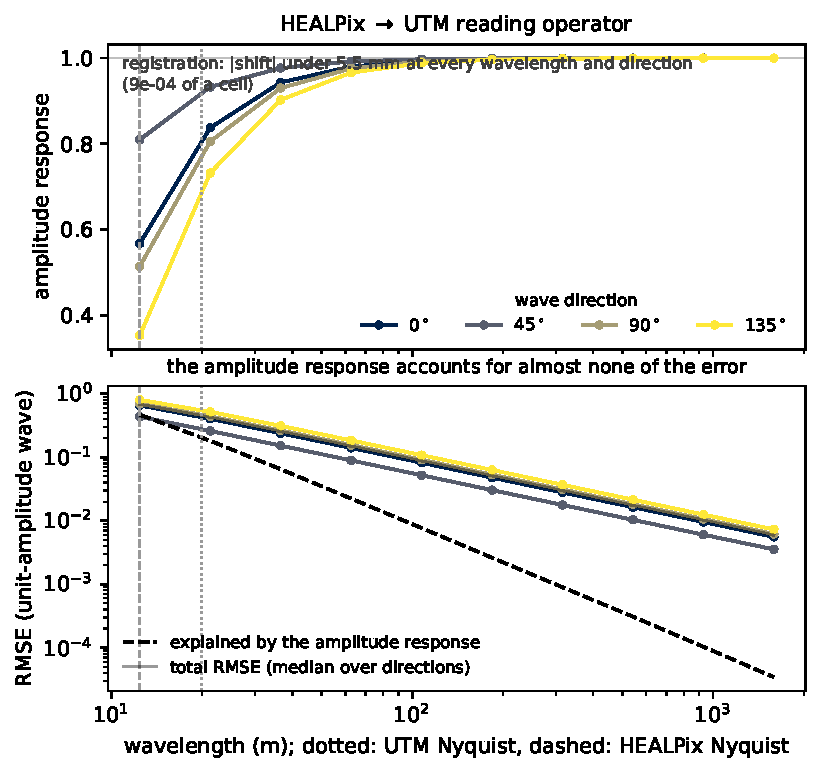
\includegraphics[width=\columnwidth]{figures/fig_operator_response}
\caption{The HEALPix$\to$UTM reading operator, measured on single-frequency
waves placed analytically on the cell centres. Top: amplitude response by wave
direction in the projected frame. Bottom: the phase of the same fit, converted
to a displacement in metres. The dotted and dashed lines mark the native and
level-20 Nyquist wavelengths. The response is well behaved and the registration
is exact, which is why the amplitude response alone is a misleading summary:
most of this operator's error is not in it (Table~\ref{tab:operator_tests} and
text).}
\label{fig:operator_response}
\end{figure}

Three things come out of it, on three regions. The operator is
registered to well under a cell: over ten wavelengths and four directions the
largest fitted displacement is \SI{2.1}{\milli\metre}, three ten-thousandths of
a cell, so there is no systematic misplacement to correct. Its
amplitude response is unremarkable ($0.99$ and above beyond \SI{100}{m},
$0.94$ at \SI{37}{m}, falling to $0.82$ near the native Nyquist and $0.53$ at
the level-20 Nyquist), and it is directional, by up to $2.29\times$ between
the $45^\circ$ and $135^\circ$ directions at the finest wavelength. That is the
first quantitative measurement in this paper of the cell-shape anisotropy that
Section~\ref{sec:resampler} invokes qualitatively.

The third is the one that matters, and it is not visible in a transfer function
at all. Regressing each projected wave on the wave itself leaves a residual that
the amplitude-and-phase model does not describe, and that residual is
\emph{almost the whole error}: it is $95\%$ of the RMSE at \SI{21}{m} and rises
to essentially $100\%$ at every wavelength above \SI{60}{m}, where the amplitude
response is already $0.98$ or better. Reading the containing cell is not a
filter; it is a sub-pixel position jitter. The ramp test gives its size
directly: a linear field is reproduced with an RMS error of $0.34$ cells of
gradient (against $0.289$, the value a uniform read anywhere within
$\pm$ half a cell would give), which is a positional jitter of about
\SI{2.1}{m} on a \SI{10}{m} native pixel. A single cell lights exactly one
native pixel in two of the three regions and \emph{none} in the third, since a
\SI{6.2}{m} cell need not contain any \SI{10}{m} pixel centre: this operator can
drop a stored cell entirely.

\subsection{Codec Audit}
\label{app:codec_audit}
Two caveats matter for the codec ranking of Section~\ref{sec:codec_choice} and the same-codec comparison of Section~\ref{sec:same_codec}. Reaching them required extending the JPEG~XL sweep beyond its quality-level ladder, which saturates near RMSE $10^{-3}$ on Sentinel-2 B04: without additional Butteraugli-distance operating points, JPEG~XL is simply absent from the high-fidelity targets and would appear to win or lose them by default. The same shift towards JPEG~2000 and JPEG~XL at aggressive compression is observed on the \emph{native UTM} side, a grid with no HEALPix quadtree structure at all, so we read it as a general property of these codecs on natural imagery (Section~\ref{sec:why_quadtree}) rather than as evidence for a HEALPix-specific advantage.

\begin{table*}[t]
\centering
\caption{Byte and type audit of the codec adapters}
\label{tab:byte_audit}
\footnotesize
\begin{tabular}{llccrc}
\toprule
Codec & Library & Self-cont. & Sidecar (B) & 16-bit floor & Bit-exact \\
\midrule
\texttt{dwt\_zstd} & pywt~1.8.0 & no & 0 & -- & -- \\
\texttt{jpeg2000\_lossless} & imagecodecs~2025.8.2 & no & 8 & $5.7\times10^{-6}$ & yes \\
\texttt{jpeg2000\_lossy} & PIL~12.0.0 & no & 8 & $5.7\times10^{-6}$ & -- \\
\texttt{jpegxl\_lossless} & imagecodecs~2025.8.2 & no & 8 & $5.7\times10^{-6}$ & yes \\
\texttt{jpegxl\_lossy} & imagecodecs~2025.8.2 & no & 8 & $5.7\times10^{-6}$ & -- \\
\texttt{sz3} & pysz~1.0.3 & no & 0 & -- & -- \\
\texttt{uncompressed} & numpy~2.3.4 & no & 0 & -- & yes \\
\texttt{zfp} & zfpy~1.0.1 & yes & 0 & -- & -- \\
\bottomrule
\end{tabular}

\end{table*}


A note on what ``lossless'' means here, and on the byte accounting behind every
number in this section; Table~\ref{tab:byte_audit} reports it. Every operating
point was written to a file, closed, re-opened and decoded by a reader written
independently of the encoder. Over 424 audited points (two regions, both
grids, both input scenarios, the full sweeps) the re-read bytes were
identical to those written, and the independently decoded array was identical
to the encoder's to the last bit. The sizes reported throughout this paper are
therefore the sizes of files that exist and can be read back, not byte counts
asserted in memory.

Three qualifications follow from that audit rather than from assumption. First,
only ZFP writes a self-contained file: every other point needs metadata carried
out of band, and for the image codecs that metadata is a float32 minimum and
span (eight bytes the reported sizes do not charge, at most $0.17\%$ of the
smallest size reported here), while the DWT baseline charges four bytes for a
scale it does not in fact write. Second, ``lossless'' JPEG~2000 and JPEG~XL are
bit-identical to the 16-bit renormalization they are handed, at all twelve
audited points, and to nothing else: not one is bit-identical to the array fed
in, under either input scenario. That renormalization imposes a floor of
$5.7\times10^{-6}$ in median, equal on both grids, which is why we write
\emph{lossless after requantization} throughout and why no operating point of
any codec goes below it. The floor sits more than an order of magnitude under
the tightest target reported here, so it does not affect the comparisons above,
but any target at or below it would be unreachable by construction. Third, the
byte counts depend on the input type, which is why the audit ran every codec
twice: once on the float32 cube, once on the integer digital numbers Sentinel-2
L2A is distributed as. The image codecs are nearly indifferent, within $0.3\%$,
because they renormalize internally; lossless JPEG~XL is $34\%$ \emph{smaller}
on integers; and the two absolute-error codecs move by two orders of magnitude,
because an error bound of $10^{-5}$ means one thing on reflectance in $[0,1]$
and quite another on digital numbers in $[0,10^{4}]$. Both grids are fed
identically everywhere in this paper, so no comparison reported here is
affected, but a reader re-running these sweeps on integer input will not
reproduce the ZFP and SZ3 curves unless the error bounds are rescaled with the
data, and we state the input units for that reason.

A fourth observation from the audit belongs to the grid comparison rather than
to the codecs. Converting to integer digital numbers costs the native UTM crop
essentially nothing (its values already sit on the DN lattice, within
$4\times10^{-9}$ to $9\times10^{-8}$ RMSE), whereas it costs the HEALPix
carrier $2.9\times10^{-5}$, the uniform quantisation error of the $10^{-4}$
step, because Clough--Tocher interpolation places the carrier's values off that
lattice. An archive that stores integer DN, as Sentinel-2 does, must therefore
either keep the carrier in floating point or accept a quantisation the native
product never pays. At $29\%$ of the tightest target reported here this is not
decisive, but it is not negligible, and it is a cost of the transfer step rather
than of the grid.

\subsection{What the Verdict Owes to Censored Sweep Points}
\label{app:censoring}
A target that the coarsest setting of a codec already satisfies is met, but
not measured: the size of that setting bounds what the codec could have
reached with a coarser one. An earlier version of this study kept such
bounds in the paired tests as if they were estimates, and at the loosest
RMSE target the oracle codec was censored in this way on 16 of the 40
regions, a share large enough that the sign of the verdict there rested on
how the bounds were read. Every ladder was therefore extended at its coarse
end (Section~\ref{sec:codecs}) and the rule of
Section~\ref{sec:rd_protocol} adopted, under which a censored pair is
excluded and counted rather than bounded. Table~\ref{tab:censoring} reports
what the verdict would be under three readings of the extended sweeps: the
ratios with every censored pair kept as a bound, the ratios on the
qualifying pairs alone (the values reported in the paper), and the interval
that bounds the median of all 40 regions once each censored value is taken
in the only direction it can move. At every reported target the three
readings agree in sign, the two medians differ by at most $0.01$, and the
interval lies on one side of parity except at $3\times10^{-3}$, where the
paper reports no verdict. The sign test in the last column assigns every
region censored on both grids to the side least favourable to the reported
verdict; it separates the grids at every reported target but
$3\times10^{-3}$. The regions that remain censored at $10^{-2}$ after the
extension are those whose contrast does not exceed the target: no codec
setting can be coarser than a constant, and for those regions the
comparison has no content.

\begin{table*}[t]
\centering
\caption{Sensitivity of the matched comparisons to censored sweep points}
\label{tab:censoring}
\footnotesize
\begin{tabular}{@{}lrrrrlrr@{}}
\toprule
Target & Bracketed & \multicolumn{3}{c}{Median ratio at $\gamma_{\mathrm{tile}}{=}1.3$} & Median & Sure & Sign $p$ \\
\cmidrule(lr){3-5}
 & regions & reported & bracketed & $p^{\mathrm{Holm}}$ & interval & HPX / UTM / ? & (worst case) \\
\midrule
RMSE $10^{-4}$ & 40 / 40 & 1.59 & 1.59 & $<10^{-4}$ & [1.59, 1.59] & 1 / 39 / 0 & $<10^{-4}$ \\
RMSE $3\times10^{-4}$ & 40 / 40 & 1.49 & 1.49 & $<10^{-4}$ & [1.49, 1.49] & 3 / 37 / 0 & $<10^{-4}$ \\
RMSE $10^{-3}$ & 39 / 40 & 1.23 & 1.23 & 0.016 & [1.22, 1.23] & 12 / 27 / 1 & 0.038 \\
RMSE $3\times10^{-3}$ & 37 / 40 & 0.91 & 0.92 & 0.137 & [0.87, 0.93] & 23 / 15 / 2 & 0.430 \\
RMSE $10^{-2}$ & 32 / 40 & 0.73 & 0.72 & $<10^{-4}$ & [0.69, 0.74] & 32 / 2 / 6 & $2\times10^{-4}$ \\
Budget 10\% & 37 / 40 & 4.02 & 4.01 & $<10^{-4}$ & [4.02, 4.04] & 0 / 39 / 1 & $<10^{-4}$ \\
Budget 5\% & 39 / 40 & 1.33 & 1.33 & $<10^{-4}$ & [1.33, 1.34] & 0 / 39 / 1 & $<10^{-4}$ \\
Budget 2\% & 40 / 40 & 0.83 & 0.83 & $<10^{-4}$ & [0.83, 0.83] & 34 / 6 / 0 & $<10^{-4}$ \\
\bottomrule
\end{tabular}
\end{table*}


\section{Reading a Target Against the Error the Product Already Carries}
\label{app:error_budget}\label{sec:error_budget}
An RMSE target is not interpretable on its own. Whether $3\times10^{-3}$ is an
aggressive or a conservative place to compress depends on how far the stored
product already sits from whatever it claims to represent, and that distance is
not the same quantity for the two transfers this study cares about.
Clough--Tocher piecewise-cubic interpolation is used here as a smooth
interpolant intended to reproduce the \emph{observed} field (the scene as
the instrument's response left it) without explicit deconvolution; it is not
structure-preserving in any absolute sense, and Section~\ref{sec:transfer_cost}
measures what it does to the spectrum. A PSF-aware transfer of the kind
the companion study proposes~\cite{delouis2026resample} represents the
\emph{latent} field, the scene before the response blurred it; it restores
small-scale structure by construction, and so hands the codec a product with
more high-frequency content to pay for. Scoring the two at the same absolute
RMSE compares errors on two different quantities, and any compression verdict
built on that comparison inherits the confusion. This section measures each
transfer against the reference it is answerable to, and then re-expresses the
results of Section~\ref{sec:results} in units of that error.

The measurement has to be synthetic, because the latent field is not
observable. For each region we build an analytic random field from that
region's own fitted spectral slope and response width
(Section~\ref{sec:support_controls}), convolve it exactly (per plane-wave
mode, so no discretised kernel enters) with that response. The width is an
effective parameter of a spectral model, fitted jointly with the slope and
partly degenerate with it, not an independent measurement of the instrument's
point-spread function; it is used here to make the synthetic field resemble the
imagery, which is all the argument requires,
and sample the result at the native pixel positions to obtain the observation.
The truth at each carrier cell is the average of the field over that cell's
sixteen level-22 children, which is the cell-average estimand the companion
study reconstructs rather than a point sample; a reconstruction agrees $2.36$
to $2.52$ times better with a cell-average reference than with a point-sample
one in that study, so mixing the two would dominate anything measured here.
Averaging four level-21 children instead moves the blur by $2\%$ and the
recovery fraction by less than a point, so the depth of the average is not a
free parameter of this comparison; we report the matched depth. Sensor noise is not optional in this
experiment. A deconvolving transfer amplifies noise exactly as it amplifies
structure, and it does so at the high frequencies a codec pays most for, so a
noiseless synthetic field favours such a transfer twice, once on
reconstruction error and again on compressibility. We add white noise at the
level Immerkaer's $3\times3$ estimator reads off each region's own imagery,
whose mask annihilates local quadratics and therefore responds to noise rather
than to scene structure; the level is $6.2$--$13.4\%$ of the field's standard
deviation by class. The damping is $\lambda=10^{-3}$, the value the companion
study reports its results at.

\begin{table*}[t]
\centering
\caption{What each transfer costs against the reference it answers to}
\label{tab:resampling_error}
\footnotesize
\begin{tabular}{@{}lrrr rrr rr@{}}
\toprule
 & \multicolumn{3}{c}{Scene} & \multicolumn{3}{c}{RMSE} & \multicolumn{2}{c}{\texttt{psf} recovery (\%)} \\
\cmidrule(lr){2-4}\cmidrule(lr){5-7}\cmidrule(lr){8-9}
Class & $\beta$ & FWHM (m) & Noise (\%) & Blur & \texttt{clough\_tocher} & \texttt{psf} & measured & noiseless \\
\midrule
Agriculture & 2.09 & 11.9 & 6.3 & 0.0088 & 0.0028 & 0.0092 & -2.5 & +13.8 \\
Forest & 2.35 & 10.1 & 7.7 & 0.0021 & 0.0019 & 0.0044 & -54.8 & -3.5 \\
Urban & 1.23 & 13.7 & 13.4 & 0.0404 & 0.0081 & 0.0405 & +3.5 & +15.6 \\
Water & 1.90 & 11.9 & 7.7 & 0.0024 & 0.0011 & 0.0032 & -12.8 & +14.0 \\
\bottomrule
\end{tabular}

\end{table*}


Table~\ref{tab:resampling_error} gives the result. Clough--Tocher's error
against the observed field is small ($5.0\%$ to $11.0\%$ of a scene's
standard deviation, median $1.9\times10^{-3}$ in reflectance) and is
dominated by the noise it faithfully transfers rather than by the interpolation
itself, which the noiseless control puts at $0.8\%$ to $1.5\%$ of the standard
deviation. Its error against the \emph{latent} field is an order of magnitude
larger, $1.6\times10^{-2}$ in median, because a transfer that does not
deconvolve leaves the whole instrument blur in place: that blur is $18.2\%$ of
the latent standard deviation over forest and $66.9\%$ over urban scenes, the
spread following the fitted slope, since a shallower spectrum puts more of the
scene's variance in the band the response attenuates. These are the two
denominators, and they differ by roughly an order of magnitude, so which one
applies is a question the paper has to put to the reader rather than settle
silently. The strict reading is the first: Clough--Tocher promised the observed
field and delivered it to $1.9\times10^{-3}$. The operative reading for a DGGS
archive is often the second, because a reader who treats the HEALPix cube as
``the data'' is comparing it to the scene, not to the observation, and is
already carrying the blur whether or not anyone accounts for it.

\begin{table*}[t]
\centering
\caption{The storage verdict against the error the product already carries}
\label{tab:alpha_budget}
\footnotesize
\begin{tabular}{@{}lrrc rrr rrr@{}}
\toprule
 & \multicolumn{3}{c}{Crossover} & \multicolumn{3}{c}{Own estimand} & \multicolumn{3}{c}{Latent scene} \\
\cmidrule(lr){2-4}\cmidrule(lr){5-7}\cmidrule(lr){8-10}
Class & Target & HPX/UTM & HPX wins & $e_{\mathrm{resample}}$ & $\kappa$ & Infl.\ \% m.\ (o.) & $e_{\mathrm{resample}}$ & $\kappa$ & Infl.\ \% m.\ (o.) \\
\midrule
Agriculture & $0.01$ & 1.20 & no & 0.0019 & 5.14 & --- (423.9) & 0.0159 & 0.63 & --- (18.0) \\
Forest & $0.01$ & 1.23 & no & 0.0013 & 7.60 & --- (666.5) & 0.0060 & 1.68 & --- (95.2) \\
Urban & $0.01$ & 0.98 & yes & 0.0063 & 1.59 & 40.4 (87.7) & 0.0753 & 0.13 & 2.5 (0.9) \\
Water & $0.01$ & 1.02 & no & 0.0007 & 14.46 & --- (1349.5) & 0.0044 & 2.26 & --- (146.7) \\
\bottomrule
\end{tabular}
\vspace{3pt}
\begin{minipage}{\textwidth}
\footnotesize
The transfer is \texttt{clough\_tocher}, which does not deconvolve, over the 40 regions of Table~\ref{tab:benchmark_scenes}. \emph{Own estimand}: its RMSE against the observed field it claims to represent. \emph{Latent scene}: its RMSE against the unblurred scene, which for a non-deconvolving transfer is the instrument blur it does not remove, the yardstick that applies when the carrier grid is read as if it were the scene. $\kappa$ is the compression target as a fraction of that denominator. The two errors add in quadrature only if their cross term vanishes, and it does not (Appendix~\ref{app:cross_term}), so the inflation columns are the \emph{measured} growth of the product's total error, with the orthogonal value $\sqrt{1+\kappa^2}-1$ in parentheses; a dash marks a crossing beyond the range the cross-term run sampled. The target shown is the tightest reported one at which HEALPix is the smaller representation, or the loosest tested where there is none. The choice of denominator moves $\kappa$ at the crossing by a factor of 6 (2.26 against 14.46 at the most expensive class), which is why both are reported rather than one elected. Against the latent scene the crossing costs less than the transfer error itself in 2 of 4 classes; the exceptions are forest, water, whose inflation is given rather than glossed.
\end{minipage}
\end{table*}


\begin{figure*}[t]
\centering
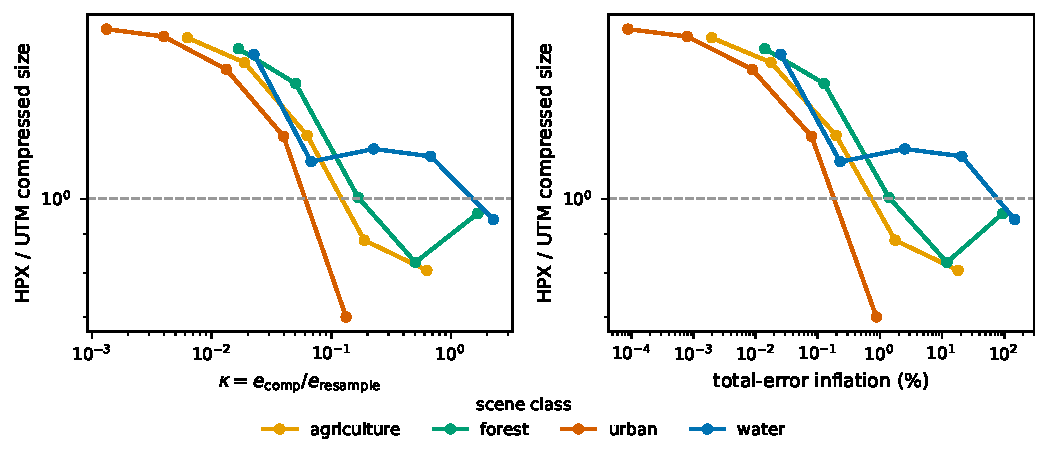
\includegraphics[width=\textwidth]{figures/fig_alpha_budget_blur.pdf}
\caption{The storage verdict as a function of what compressing costs the
product, latent-scene denominator. Left: median HPX/UTM compressed size against
$\kappa=e_{\mathrm{comp}}/e_{\mathrm{resample}}$, the compression error as a
fraction of the error the product already carries. Right: the same curves
against the resulting growth of the product's total error,
$\sqrt{1+\kappa^2}-1$. The dashed line marks parity; points below it favour
HEALPix. Three of the four classes cross parity while the compression error is
still a fraction of the transfer error. Under the own-estimand denominator the
curves are unchanged in shape and shifted right by a class-dependent factor of
$4.7$ to $12.3$, which is the ratio of the two denominators in
Table~\ref{tab:alpha_budget}.}
\label{fig:error_budget}
\end{figure*}

Table~\ref{tab:alpha_budget} and Fig.~\ref{fig:error_budget} restate the
crossovers of Section~\ref{sec:results} in these units. Write
$\kappa = e_{\mathrm{comp}}/e_{\mathrm{resample}}$ for the compression error as
a fraction of the error already carried. How the two combine is a measurement
and not an identity: in general
$D_{\mathrm{total}}/D_0=\sqrt{1+\kappa^2+2\rho\kappa}$ with $\rho$ their
normalised inner product, and the familiar $\sqrt{1+\kappa^2}-1$ is its
$\rho=0$ case. Appendix~\ref{app:cross_term} measures $\rho$ and finds it is
neither zero nor of one sign, so the inflation reported here is the measured
one, with the orthogonal value beside it for reference. The crossover target itself is a property of the ratios and so is
common to both denominators; what the denominator changes is what reaching it
costs. Against the latent scene, HEALPix becomes the smaller representation at
$\kappa=0.13$ over urban scenes and $\kappa=0.19$ over agriculture (total
error inflated by a measured $2.5\%$ and $5.1\%$ for a $30\%$ and a $12\%$
saving in bytes) and at $\kappa=0.50$ over forest, for $16.0\%$ inflation
and a $17\%$ saving. Each of those is about twice what the orthogonal formula
would give ($0.9\%$, $1.8\%$, $11.9\%$), for the reason
Appendix~\ref{app:cross_term} sets out. Water is the exception in both readings: its crossing arrives only at
the loosest tested target, where the compression error is more than twice the
transfer error, and the $6\%$ saving there is too small to be meaningful. Against the
own estimand the same three crossings cost $\kappa=1.54$, $1.59$ and $2.28$,
i.e.\ measured inflations of $37\%$, $40\%$ and $115\%$ ($84\%$, $88\%$ and
$149\%$ under the orthogonal formula, which overstates them here for the
reason Appendix~\ref{app:cross_term} sets out): on that yardstick no
crossing is cheap.

That asymmetry is the substantive finding of this section, and it sharpens the
conditional conclusion of Section~\ref{sec:common_reference} rather than
softening it. For a product used as an information-preserving copy of the
scene (the case in which the blur is already part of what the reader
tolerates), the regime where HEALPix becomes the cheaper representation is
reached while the compression error is still a small fraction of the error the
product carries anyway, for three of the four scene classes. For a product held
to the observation it was made from, it is not. The same measurement therefore
supports both the optimistic and the pessimistic reading, and the choice
between them is a statement about the intended use of the archive, not about
the grid.

The deconvolving transfer does not yet support the same accounting, and we
report the reason rather than the number we hoped for. In this harness the
PSF-aware reconstruction recovers essentially none of the blur at the measured
noise level ($-7.7\%$ to $-1.2\%$ by class, positive in only 16 of 40
regions) and a small but systematic $+3.0\%$ to $+6.5\%$ in a
noiseless control at the same averaging depth, positive in 39 of 40 regions.
The companion study reports $15.4\%$ to
$19.6\%$, noise-free, under the same recovery definition and the same damping.
The gap is not explained by an easier inverse problem on their side: their
synthetic observation is averaged over a \SI{10}{m} square detector aperture
that the scalar Gaussian inverse does not model, a mismatch they state
explicitly, and which makes their recovery conservative rather than flattered.
What we can identify on ours is threefold. The noise is the largest term: a
deconvolution amplifies it preferentially at exactly the frequencies it is
trying to restore, which is why our own noiseless control moves from
approximately zero to $+5.4\%$ in median. The latent field is the second: a power law
extrapolated to the level-20 Nyquist places $2.3\%$ (forest) to $31.1\%$
(urban) of the latent variance above the \emph{native} Nyquist, in a band the
fitted response attenuates to a few percent of its amplitude, so most of the
blur we charge is not recoverable by any damping, which is also why the blur
is $18$ to $67\%$ of the latent standard deviation here, and why urban scenes,
with the shallowest fitted slope, recover least. A third candidate, the depth
of the cell average, we tested and can exclude: matching the companion's
sixteen level-22 children rather than four at level 21 moves the recovery
fraction by less than a point. A residual gap remains after the two that do
matter, and we do not attribute it. The consequence for this paper is the same either
way: the super-resolution surcharge (what a deconvolved product costs to
store at equal $\kappa$) cannot be quantified from the present
measurements, and we list it as the outstanding item rather than estimate it
(Section~\ref{sec:limitations}).


\section{Is the Compression Error Orthogonal to the Transfer Error?}
\label{app:cross_term}\label{sec:cross_term}
Converting a compression target into a growth of the product's total error, as
Appendix~\ref{app:error_budget} does, needs to know how the two errors combine.
Writing $e_0 = x - \text{truth}$ for the transfer error on the carrier cells,
$e_c = \tilde{x} - x$ for the compression error, and noting that
$e_0 + e_c = \tilde{x} - \text{truth}$, the exact relation is
\begin{equation}
\frac{D_{\mathrm{total}}}{D_0} = \sqrt{1 + \kappa^2 + 2\rho\kappa},
\qquad \rho = \frac{\langle e_0, e_c\rangle}{D_0 D_c},
\label{eq:cross_term}
\end{equation}
of which quadrature is the $\rho = 0$ case. The difference is not cosmetic: at
$\kappa=0.5$, $\rho=-1$ would \emph{halve} the product's error and $\rho=+1$
would grow it by half. We therefore measure $\rho$ rather than assume it, on
the synthetic scene of Appendix~\ref{app:error_budget} so that both errors are
available exactly, with both taken on the same level-20 cells and in the same
norm, which a comparison made after projecting to UTM would not give either.

\begin{table*}[t]
\centering
\caption{Cross term between the transfer and compression errors}
\label{tab:cross_term}
\footnotesize
\begin{tabular}{@{}lllrrrrr@{}}
\toprule
Transfer & Reference & $\kappa$ & $n$ & median $\rho$ & $[10,90]\%$ & Measured (\%) & Quadrature (\%) \\
\midrule
\texttt{clough\_tocher} & latent & $0.1$ & 66 & +0.001 & [-0.01, +0.07] & +0.6 & +0.5 \\
\texttt{clough\_tocher} & latent & $0.2$ & 93 & +0.063 & [-0.00, +0.19] & +3.4 & +2.3 \\
\texttt{clough\_tocher} & latent & $0.5$ & 148 & +0.213 & [+0.01, +0.34] & +20.4 & +12.9 \\
\texttt{clough\_tocher} & latent & $1$ & 248 & +0.274 & [-0.01, +0.35] & +57.5 & +43.5 \\
\texttt{clough\_tocher} & observed & $0.1$ & 37 & +0.000 & [-0.00, +0.00] & +0.4 & +0.4 \\
\texttt{clough\_tocher} & observed & $0.2$ & 59 & -0.001 & [-0.05, +0.00] & +1.9 & +2.4 \\
\texttt{clough\_tocher} & observed & $0.5$ & 77 & -0.124 & [-0.23, -0.00] & +10.5 & +16.2 \\
\texttt{clough\_tocher} & observed & $1$ & 118 & -0.147 & [-0.48, -0.02] & +26.3 & +40.7 \\
\bottomrule
\end{tabular}

\end{table*}


\begin{figure*}[t]
\centering
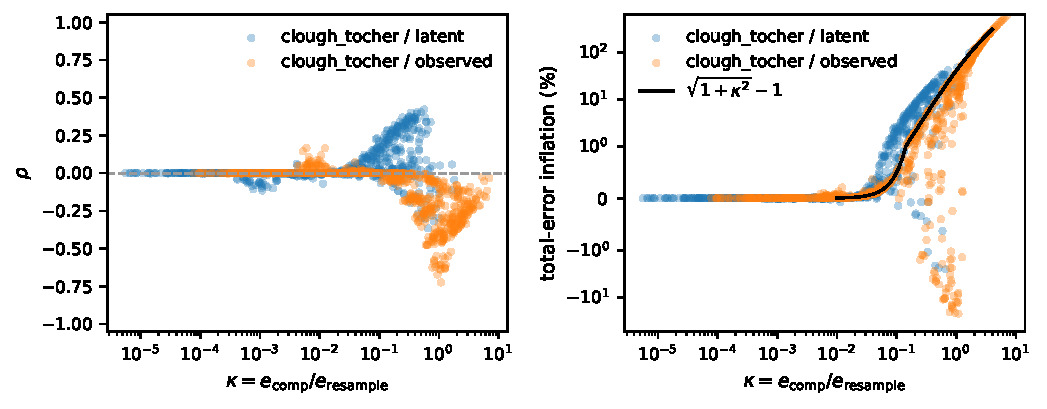
\includegraphics[width=\textwidth]{figures/fig_cross_term.pdf}
\caption{The cross term, per operating point, over 40 regions and two codec
families. Left: $\rho$ against $\kappa$. Right: the measured growth of the
product's total error against $\kappa$, with $\sqrt{1+\kappa^2}-1$ drawn as the
orthogonal case. The four series are the two reference fields crossed with the
two codecs; the wavelet coder carries the whole effect under both references
and in opposite directions, while the block-floating-point coder sits on the
orthogonal curve.}
\label{fig:cross_term}
\end{figure*}

Table~\ref{tab:cross_term} gives the result, and the sign depends on which
reference the product is held to, the same distinction that organises
Section~\ref{sec:common_reference} and Appendix~\ref{app:error_budget}, arriving here
for a mechanical reason. Against the \emph{observed} field, $\rho$ is negative
and grows in magnitude with $\kappa$, reaching $-0.33$ at $\kappa=1$: the
transfer error is there dominated by the sensor noise the transfer faithfully
carried; it is what takes Clough--Tocher from $0.8$--$1.5\%$ of a scene's
standard deviation without noise to $5.0$--$11.0\%$ with it
(Table~\ref{tab:resampling_error}), and a lossy coder discards part of that
noise along with everything else it discards at high frequency. The two errors
partly cancel, and quadrature \emph{overstates} the damage, by $11$ percentage
points at $\kappa=0.5$ and $24$ at $\kappa=1$. Against the \emph{latent} scene
the sign reverses, $\rho$ rising to $+0.17$ at $\kappa=0.2$: there the transfer
error is essentially the blur the transfer did not remove, which is a
\emph{deficit} of high-frequency content, and a wavelet coder's error is
another such deficit. The two align, the errors add faster than in quadrature,
and the orthogonal formula \emph{understates} the inflation, by $2.5$
percentage points at $\kappa=0.2$ and $6.6$ at $\kappa=0.5$, which is roughly a
factor of two on the figures Appendix~\ref{app:error_budget} reports.

What makes this a mechanism rather than a coincidence is the codec that does
not participate. Splitting Fig.~\ref{fig:cross_term} by codec, the wavelet
coder carries the entire effect ($\rho = -0.18$ against the observed field
and $+0.16$ to $+0.29$ against the latent scene at the crossing values of
$\kappa$) while ZFP, whose block-floating-point quantisation does not sort
by spatial frequency, stays orthogonal under both references
($|\rho| \le 0.03$) and reproduces $\sqrt{1+\kappa^2}-1$ to a few tenths of a
percentage point. The cross term is thus not a property of compression in
general but of coders that discard by frequency, which is what the transfer
error of a non-deconvolving transfer is made of at either reference.

Two limits on this measurement. The \emph{sign} of $\rho$ follows from both
errors being high-frequency deficits, or from one being noise the other
removes, and neither depends on the details of the synthetic field; its
\emph{magnitude} does, because the blur here is an exact Gaussian attenuation
of a power law rather than whatever a real instrument response leaves behind.
And the sampled range of $\kappa$ against the latent scene stops short of the
water class's crossing at $\kappa=2.26$, which is why
Table~\ref{tab:alpha_budget} reports no measured inflation there rather than an
extrapolation. Neither limit affects the practical conclusion, which is that
the inflation figures of Appendix~\ref{app:error_budget} must be measured rather
than computed, and that the direction of the error one makes by computing them
depends on the reference the product answers to.


\section{Detailed Limitations}
\label{app:limitations}
\begin{itemize}
    \item \textbf{The verdict is conditional on the transfer, by about a factor of two, and the transfer this paper uses is the most favourable of those tested.} Section~\ref{sec:transfer_cost} measures this rather than leaving it open: rebuilding the carrier with a PSF-aware or an
inverse-distance transfer costs $1.2$ to $2.4$ times the bytes at the same coding RMSE relative to each transfer's own uncompressed carrier, which is more than the margin by which HEALPix leads at the loosest targets, so under either of them it leads at none. Clough--Tocher is also the most accurate of the transfers tested against an analytic field, and we argue the two properties share a cause, but the argument does not extend the result to transfers we have not swept (the original inverse-distance weighting among them) and it does not make the reported ratios properties of the grid. One residual gap remains in this ablation (the accuracy column of Table~\ref{tab:kernel_ablation} now covers the 40 regions, and the inverse-distance resampler that Section~\ref{sec:resampler} replaced is the \texttt{linear} row of that table and the IDW control of Section~\ref{sec:transfer_cost}): we have not tested a non-deconvolving transfer of Clough--Tocher's smoothness class, which is what would isolate deconvolution from smoothness properly rather than bounding it as we do;
    \item \textbf{An earlier out-of-range figure for the inverse-distance transfer was a diagnostic artefact.} A previous version of Section~\ref{sec:transfer_cost} reported that the inverse-distance average placed $0.95\%$ of cells outside the range of its input and read this as overshoot. The range had been taken over the observation restricted to the two footprints' intersection while the values were taken over the whole tile, about a fifth of which lies outside that mask, so a cell could sit outside the range with no overshoot at all, and a transfer whose kernel reaches further collected more such cells. The diagnostic now takes both over the same ground; the argument of Section~\ref{sec:transfer_cost} rests on the transfer error of Table~\ref{tab:kernel_ablation}, which is unaffected.
    \item \textbf{The equal-area UTM square is not pixel-for-pixel identical to the HEALPix footprint.} As noted in Section~\ref{sec:utm_crop}, the axis-aligned $637\times637$ UTM square extends slightly beyond the rotated HEALPix diamond along its edges and falls slightly short of it at the north/south/east/west corners. It matches the HEALPix tile's ground \emph{area} exactly (both grids being fixed-size representations, Table~\ref{tab:storage_accounting}), but not its exact shape; a polygon-masked, footprint-exact crop remains a possible further refinement, though we do not expect it to materially change the fixed $2.58\times$ oversampling relationship, which follows from HEALPix's equal-area property rather than from the crop shape;
    \item \textbf{The overhead is reported as a parameter because only its container component is measured.} Section~\ref{sec:results} now reports the verdict over a continuous range of the overhead \emph{ratio} $\gamma=\gamma_{\mathrm{UTM}}/\gamma_{\mathrm{HPX}}$ rather than at one value, so no conclusion here depends on choosing $1.30$, and the container cost of each side is measured at under half a percent. What remains assumed is granule geometry, which we have not measured on complete Sentinel-2 products. The following remains true of that assumption:
     UTM is a coordinate reference system; padding, overlap, and per-tile metadata are properties of a particular product organisation (here, Sentinel-2's MGRS granule layout), and a native UTM COG or Zarr archive need not carry this overhead at all. We report the $\gamma_{\mathrm{tile}}=1$ result as the overhead-free carrier/native comparison, which still includes the transfer, and the $\gamma_{\mathrm{tile}}=1.30$ result as one illustrative operational scenario (Table~\ref{tab:gamma_continuous} reports the critical overhead $\gamma_\star$ directly, so the conclusion at any other assumed overhead can be read off without rerunning the analysis). We have not measured $\gamma_{\mathrm{tile}}$ from real, complete tiled product files in this study, nor swept it continuously over $[1.0,1.5]$ for the matched-budget protocol (Table~\ref{tab:error_at_size}); both are left for future work. For compressed storage (Section~\ref{sec:overhead}), we further assume the overhead applies proportionally to the compressed byte count, i.e.\ that the padded/overlapping fraction of a native tile compresses at roughly the same ratio as the tile itself; this is a simplifying assumption, not a measurement of real, complete tiled product files;
    \item \textbf{The level-19 comparison is made on a cell-averaged carrier, not on a directly evaluated one.} Section~\ref{sec:level_choice} aggregates the stored level-20 tile in groups of four, which is the exact quadtree Haar transform and therefore the cell-average of the carrier over each level-19 cell. The carrier holds point evaluations of the Clough--Tocher interpolant at cell centres, and for a general interpolant the parent-centre value is not the mean of the four child-centre values, so the aggregate is a level-19 carrier built by interpolation followed by averaging rather than the one the same transfer would have produced at that level. The quantities reported there are exact for the object measured and bound rather than reproduce the direct carrier; evaluating the same interpolant at the level-19 cell centres, reading it back through the same operator and sweeping it is the experiment that would settle the level choice, and it has not been run;
    \item \textbf{The loosest targets are established on fewer regions.} A (region, target) pair enters a paired test only when the codec the oracle selects brackets the target with two measured points on both grids, so that no bound is tested as if it were an estimate (Section~\ref{sec:rd_protocol}, Appendix~\ref{app:censoring}). After the ladders were extended at their coarse end, the pairs that fail are the lowest-contrast scenes, for which the target is a large fraction of the standard deviation of the scene itself: none at the two tightest RMSE targets, one at $10^{-3}$, three at $3\times10^{-3}$ and eight at $10^{-2}$, so that the verdict at the loosest target rests on 32 regions rather than 40, with no urban scene among the absent. We report exact two-sided Wilcoxon $p$-values on log-ratios together with a Holm correction across the full eight-test family; seven of eight survive it. The exception, the $3\times10^{-3}$ RMSE target, is the crossover point itself and is reported as inconclusive rather than as evidence of equivalence, since no equivalence margin has been defined. The two most generous storage budgets ($40\%$ and $20\%$ of the raw tile) qualify on $0\%$ and $65\%$ of the regions and are withheld entirely;
\item \textbf{Neither reconstruction reference is the whole story.} Section~\ref{sec:results} scores each grid against its own raw representation and Section~\ref{sec:common_reference} scores both against the same observation; the two disagree at the crossover, and we report both rather than electing one. The floor of Table~\ref{tab:representation_floor} is the error of a Clough--Tocher tile read at nearest cell, and Section~\ref{sec:operator} shows the read alone is large enough to account for a floor of that size, so the floor is an upper bound on what the representation costs rather than a measurement of it. The decomposition is now half done: a reconstructor that interpolates within the carrier raster removes two thirds of the floor's variance (Table~\ref{tab:reader_floor}), and the PSF-aware transfer of the companion study~\cite{delouis2026resample} has been run through the same protocol (Section~\ref{sec:transfer_cost}). The common-reference sweep of Section~\ref{sec:common_reference} has been re-scored through the interpolating read (Table~\ref{tab:common_two_readers}) and its verdict reported under both; what remains open is the $3\times10^{-3}$ target, bracketed for $57\%$ of regions under the better read and therefore still withheld, and a read matched to the PSF transfer on the PSF tiles, which Table~\ref{tab:reader_floor} shows to be within $4\%$ of the interpolating one;
    \item \textbf{The super-resolution surcharge is measured, but our deconvolution control does not reproduce the companion's recovery, so the product it prices is not the one that study validates.} Section~\ref{sec:transfer_cost} prices the deconvolved carrier at $1.27$ to $2.19$ times the Clough--Tocher one, of which only a few percent is attributable to deconvolving rather than to leaving Clough--Tocher's smoothness class. That is a measurement on real imagery and does not depend on the synthetic harness. What does depend on it is the claim that the extra bytes buy a better estimand: in our harness the PSF-aware reconstruction recovers $+3.0\%$ to $+6.5\%$ of the blur without noise and nothing at the measured noise level, against the $15.4\%$ to $19.6\%$ the companion study reports noise-free. We identify the added noise and a latent spectrum extrapolated to the level-20 Nyquist as contributors, exclude the depth of the cell average by measurement, and are left with a residual gap we cannot attribute. The storage price is therefore reportable and the quality it purchases is not, which is the asymmetry a reader should carry away rather than a net verdict on PSF-aware carriers;
    \item \textbf{The oracle-best-codec comparison is an envelope, and the crossover is codec-dependent.} Tables~\ref{tab:storage_at_rmse}--\ref{tab:error_at_size} select the best-performing codec independently per region and per grid at each target, which is the best rate--distortion envelope attainable from the tested family and not an operational archive. Section~\ref{sec:same_codec} reports the controlled comparison with the codec held fixed: four of the five codecs reproduce the regime-dependent pattern, so codec selection is not what produces the crossover, but ZFP does not reproduce it at all, so the crossover is a property of the carrier under a rate-adaptive transform coder rather than of the carrier alone. The same-codec comparison should be read as the operational result and the oracle protocol as an upper bound on what codec selection could add;
    \item \textbf{The byte and type audit covers two regions, not forty.} Table~\ref{tab:byte_audit} reports, per encoded point, the library and version, the input dtype and scaling, the pre-codec conversion error, payload against reported bytes, and a bit-identity test, over two regions on both grids under both input scenarios. It found no gap between reported and on-disk sizes and no disagreement with an independent decoder at any of 424 points. Because what it tests is the adapters, which do not vary by region, we do not expect the remaining 38 to differ, but we have not run it over them, and two accounting choices it exposes stand as reported: the image codecs' eight-byte scale-and-offset sidecar is not charged to their sizes, and the DWT baseline charges four bytes for a scale it never writes;
    \item \textbf{The footprint mismatch is bounded, not eliminated, and its geometry is measured from cell centres.} Section~\ref{sec:support_controls} shows that a control with no support mismatch, no scene content and no transfer reproduces the decline of the measured gap and its magnitude to within $8$--$27\%$; the residual is not attributed to any one of the three, and none of them is removed from Tables~\ref{tab:storage_at_rmse}--\ref{tab:error_at_size}. The intersection fractions quoted in Section~\ref{sec:utm_crop} are computed from the convex hull of the cells' centres rather than from the exact cell-boundary polygon, and we have not computed each footprint's geodesic area scene by scene;
    \item \textbf{Codecs are swept over their own native quality parameter, not a common one.} The matched-RMSE/matched-size protocol of Section~\ref{sec:rd_protocol} is designed specifically to make this comparison as fair as achievable without assuming codec-internal parameters are equivalent, but residual convention effects cannot be fully excluded;
    \item \textbf{Single band, single sensor.} Only Sentinel-2 B04 (red, \SI{10}{m}) is evaluated; extending the comparison to other bands, other resolutions, and other sensors whose native sampling also falls between HEALPix levels would strengthen the generality of the claim;
    \item \textbf{The HEALPix side uses a deliberately simple resampling.} Even after the kernel correction of Section~\ref{sec:resampler}, the Clough--Tocher piecewise-cubic interpolation used to populate the level-20 tiles is a generic, PSF-agnostic resampler, chosen to match the native UTM side's content as closely as a simple method allows, not to model the sensor's actual point-spread function. The production resampling pipeline this group is developing for operational use, a point-spread-function-aware resampler~\cite{delouis2026resample}, is expected to inject more genuine high-frequency detail into the HEALPix representation than either resampler evaluated here; since less redundant, higher-entropy content compresses less well, the HEALPix-side compression ratios reported here should be read as optimistic relative to that future operational pipeline, not as a bound on it. We previously argued that the margin was bounded from one side, on the grounds that the imagery carries only $0.21\%$ of its variance above half the native Nyquist; we withdraw that argument. Low power in the \emph{observed} field bounds nothing about the latent one, since an instrument response is precisely what attenuates it, and this study's own fitted spectra put $2.3\%$ (forest) to $31.1\%$ (urban) of the latent variance above the native Nyquist (Appendix~\ref{app:error_budget}). Quantifying the gap is future work;
    \item \textbf{No downstream-product evaluation, and B04 only.} Only reflectance RMSE is evaluated; no derived product is computed. We deliberately make no claim about how the measured errors would propagate into an index such as NDVI: that requires adding B08 and a common validity mask, and until it is done the scope of this study is one band of one sensor, as the title states. That the propagation is not negligible is documented: lossy compression of remote-sensing imagery changes downstream land-cover classification at compression ratios well inside the range studied here~\cite{zabala2011lossy}, so a reflectance RMSE budget is a necessary but not a sufficient basis for choosing an operating point;
    \item \textbf{The scope is observation data, at one epoch. Gridded model
    output is a different compression problem, not a larger instance of this
    one.} Everything measured here is a single band of a single Sentinel-2
    acquisition over a regional tile, and three of this paper's central
    constructions are properties of that setting rather than of HEALPix.
    The error budget of Appendix~\ref{app:error_budget} exists because an
    instrument response stands between the stored field and the scene; model
    output is already a cell average of a discretised field, so there is no
    transfer error to charge and no choice of estimand to make, and the
    denominator of $\kappa$ would have to be the model's own numerical error or
    the tolerance of the downstream application instead. The codec ranking of
    Section~\ref{sec:codec_choice} is a ranking of 2-D coders on one field; for
    a time-varying product the dominant redundancy is temporal, which none of
    the codecs favoured here exploits and two of the codecs ranked below them
    address by construction, so that ordering should not be assumed to carry
    over. And the oversampling factor of~\eqref{eq:alpha} is imposed by the
    \SI{10}{m} native pitch, whereas the HEALPix level of a model product is a
    free design parameter, which turns the critical overhead $\gamma_\star$
    from a verdict into a design curve. Conservation adds a constraint absent
    here entirely: a lossy operating point that meets an RMSE budget need not
    preserve an area-integrated quantity, which for flux fields is often the
    property that matters. We name this as a distinct class of problem, on
    which the present measurements have no bearing, rather than as an
    extension of the present results;
    \item \textbf{Forty regions, one tile each.} Statistical replication is one dominant level-10 tile per region. Ten regions per land-cover class and a latitude span covering both HEALPix cell-shape regimes give the per-target tests real power, but genuinely independent replicate tiles \emph{within} a region would be needed to separate scene-to-scene variability from tile-to-tile variability at a single site;
    \item \textbf{The acquisition window is not identical across regions, and ``lossless'' is not bit-exact.} Each native window is centred on the carrier tile and sized to the smallest that holds it with its halo, so window widths differ between regions; nothing measured depends on that width, but it is recorded per region rather than being uniform. Separately, the image codecs receive a 16-bit requantization of the float32 tile, giving every codec on a given grid an RMSE floor of $5.7\times10^{-6}$ in median (Table~\ref{tab:byte_audit}); the reported lossless points are verified bit-identical after that step and are not bit-identical to the original samples;
    \item \textbf{Ratios over near-constant scenes are fragile.} Over deep water at the loosest targets, compressed files fall below \SI{10}{kB}, where container overhead is a large share of the total; individual water-region ratios there range from $0.07$ to $6.1$ and are not informative, even though the class medians behave like the others. A minimum-size floor below which ratios are not reported would make this explicit;
    \item \textbf{Learned compression is not evaluated.} The five codecs here are hand-designed and general-purpose; end-to-end optimised neural codecs~\cite{balle2017endtoend} now lead the rate--distortion frontier on natural imagery and have remote-sensing and onboard variants~\cite{valsesia2019onboard}. Comparing two grids with a learned codec requires models trained symmetrically on both, since a model trained on projected imagery and applied to a Morton-de-interleaved HEALPix raster would be evaluated off its training distribution; building that pair, and separating the resulting difference from the grid effect measured here, is a study of its own. The ratios reported here should therefore be read as characterising generic codecs, not as a bound on what any codec could achieve;
    \item \textbf{Codec choice was evaluated on compression efficiency alone.} The codecs compared here also differ in how well they support the partial, range-based reads that motivate DGGS-style chunking in the first place (Section~\ref{sec:intro}): JPEG~2000's EBCOT coding and JPEG~XL's progressive/tiled modes allow a client to fetch and decode a spatial or quality sub-range of a chunk without retrieving it whole, a property shared, at the block level, by ZFP's fixed-rate encoding; SZ3 and the DWT+Zstandard baseline are not designed for partial decoding, so a client wanting part of a chunk compressed with one of them must fetch and decode it in full. If partial access is an operational requirement, the strongest compressor at a given quality (Table~\ref{tab:codec_ranking}) is not automatically the right choice, and this trade-off is not quantified here;
    \item \textbf{Global-sphere behaviour is not yet measured} and is not claimed to follow unchanged from the regional result (Appendix~\ref{app:global_sphere}).
\end{itemize}
\section{Towards Global-Sphere Compression}
\label{app:global}
\label{app:global_sphere}
All measurements in this paper use a single dominant level-10 parent tile per scene ($1024\times1024$ level-20 cells), chosen because it is large enough to amortize per-chunk codec overhead while remaining a practical chunking unit. The coarsest possible HEALPix parent is not ``level 1'' but level (order) 0: with $N_{\mathrm{pix}}(\ell)=12\cdot4^{\ell}$, level 0 has exactly the 12 base faces of the sphere ($N_{\mathrm{pix}}(0)=12$), and level 1 already has 48. A single level-0 face carried down to level 20 would contain $4^{20}\approx10^{12}$ cells -- far too large to compress as one monolithic array, and not a realistic chunking unit on its own.

A full-sphere product would therefore need a multi-chunk hierarchy -- for example, many level-10-rooted tiles per base face, each handled exactly as in this paper -- rather than one array per base face, together with explicit treatment of the 12 base-face boundaries, which are not simple raster seams. We have not measured full-sphere behaviour, and we do not claim that the regional pattern reported here extends to it unchanged; whether it does, and how base-face boundaries should be handled, is a concrete question for future work rather than a corollary of the present results. A full-sphere treatment would also open a representation the tile-local codecs used here cannot exploit: multiscale bases defined on the sphere itself, such as needlets~\cite{marinucci2008needlets}, and the sphere-adapted scattering representations already used to model non-Gaussian structure in full-sky HEALPix data~\cite{delouis2022scattering}, model exactly the cross-scale dependency that Section~\ref{sec:redundancy} identifies as the source of the compressibility, but on a support no chunk boundary interrupts.

